\documentclass[czech]{ExcelAtFIT} % Document font size and equations flushed left

\usepackage[T1]{fontenc}
\usepackage[font={normalsize}]{subfig}
\usepackage{array}
\usepackage{multirow}
\usepackage{multicol}
\usepackage{dblfloatfix}
%\newcommand{\uv}[1]{\quotedblbase #1\textquotedblleft}

\colorlet{fixme}{green!50!black}
\newcommand{\fixme}[1]{{\color{fixme} {{\textbf{[FIXME]}} #1} }}

\colorlet{sos}{red}
\newcommand{\sos}[1][]{{\color{sos} {{[ \textbf{???}} #1]} }}

\colorlet{grayintable}{black!50}

%\newcommand*{\@rowstyle}{}
\newcommand*{\rowstyle}[1]{% sets the style of the next row
    \gdef\@rowstyle{#1}%
    \@rowstyle\ignorespaces%
}

\newcolumntype{=}{% resets the row style
    >{\gdef\@rowstyle{}}%
}

\newcolumntype{+}{% adds the current row style to the next column
    >{\@rowstyle}%
}


\hyphenation{pixel}
\hyphenation{pixely}
\hyphenation{pixelu}
\hyphenation{pixelů}
\hyphenation{UsedGenes}


%--------------------------------------------------------
%--------------------------------------------------------
%	REVIEW vs. FINAL VERSION
%--------------------------------------------------------

%   LEAVE this line commented out for the REVIEW VERSIONS
%   UNCOMMENT this line to get the FINAL VERSION
\ExcelFinalCopy


%--------------------------------------------------------
%--------------------------------------------------------
%	LANGUAGE
%--------------------------------------------------------
%   Recommended language for Excel@FIT paper is English.
%   However, in emergency, you can write in Czech or Slovak.
%   In such a case, uncomment one of these lines to localize the template.
%--------------------------------------------------------
%\ExcelSlovakLabels
\ExcelCzechLabels


%--------------------------------------------------------
%--------------------------------------------------------
%	PDF CUSTOMIZATION
%--------------------------------------------------------

\hypersetup{
    pdftitle={Souběžné učení v~koevolučních algoritmech},
    pdfauthor={Michal Wiglasz},
    pdfkeywords={Keyword1, Keyword2, Keyword3}
}


%--------------------------------------------------------
%--------------------------------------------------------
%	ARTICLE INFORMATION
%--------------------------------------------------------

\ExcelYear{2015}

\PaperTitle{Souběžné učení v~koevolučních algoritmech}

\Authors{Michal Wiglasz*}
\affiliation{*%
    \href{mailto:xwigla00@stud.fit.vutbr.cz}{xwigla00@stud.fit.vutbr.cz},
    \textit{Fakulta informačních technologií, Vysoké učení technické v~Brně}}
%%%%--------------------------------------------------------
%%%% in case there are multiple authors, use the following fragment instead
%%%%--------------------------------------------------------
%\Authors{Jindřich Novák*, Janča Dvořáková**}
%\affiliation{*%
%  \href{mailto:xnovak00@stud.fit.vutbr.cz}{xnovak00@stud.fit.vutbr.cz},
%  \textit{Faculty of Information Technology, Brno University of Technology}}
%\affiliation{**%
%  \href{mailto:xdvora00@stud.fit.vutbr.cz}{xdvora00@stud.fit.vutbr.cz},
%  \textit{Faculty of Information Technology, Brno University of Technology}}

\Keywords{
Koevoluční algoritmus ---
Kartézské genetické programování ---
Genetický algoritmus ---
%Baldwinův efekt ---
Plasticita fenotypu ---
Predikce fitness ---
Obrazový filtr
}

\Supplementary{\href{http://michalwiglasz.cz/excel2015.tar.gz}{Zdrojové kódy}}
%\Supplementary{\href{http://youtu.be/S3msCdn3fNM}{Ukázkové video} --- \href{http://excel.fit.vutbr.cz/}{Zdrojové kódy}}


%--------------------------------------------------------
%--------------------------------------------------------
%	ABSTRACT and TEASER
%--------------------------------------------------------

\Abstract{
Kartézské genetické programování (CGP) se využívá zejména pro automatizovaný návrh čí\-sli\-co\-vých obvodů, ale ukázalo se být úspěšnou metodou i pro řešení jiných inženýrských úloh. Časově nejnáročnější částí výpočtu je vyhodnocení kvality kandidátních řešení. Bylo ukázáno, že evoluci je možné urychlit pomocí koevoluce s~prediktory fitness, které slouží k~přibližnému určení kvality kandidátních řešení. Nevýhodou koevoluce je nutnost provést mnoho časově náročných experimentů pro určení nejvýhodnější velikosti prediktoru pro daný problém. V~tomto článku je představena nová reprezentace prediktorů fitness s~plastickým fenotypem, založená na principech souběžného učení v~evolučních algoritmech. Plasticita fenotypu umožňuje odvodit různé fenotypy ze stejného genotypu. Díky tomu je možné adaptovat velikost prediktoru v~průběhu evoluce na obtížnost řešeného problému. Z~experimentů vyplývá, že lze dosáhnout srovnatelné kvality jako u~standardního CGP při kratší době běhu programu a zároveň odpadá nutnost hledání nejvýhodnější velikosti prediktoru.
}

\Teaser{
    \TeaserImage{filter-cgp2dimp.pdf}
}



%--------------------------------------------------------
%--------------------------------------------------------
%--------------------------------------------------------
%--------------------------------------------------------
\begin{document}

\startdocument


%--------------------------------------------------------
%--------------------------------------------------------
%	ARTICLE CONTENTS
%--------------------------------------------------------

%--------------------------------------------------------
%--------------------------------------------------------
%--------------------------------------------------------
%--------------------------------------------------------
\section{Úvod}

Genetické programování umožňuje automatizovaně vytvářet programy s~požadovaným chováním, které je definováno trénovací množinou. Každý prvek této množiny reprezentuje jeden případ fitness a skládá se ze vstupních hodnot programu a po\-ža\-do\-va\-ných vý\-stup\-ních hodnot \cite{HandbookGP}. U~složitějších problémů může být ta\-ko\-vých případů fitness velmi mnoho. Protože vý\-po\-čet fitness je časově nejnáročnější částí evoluce, je vhodné do trénovací množiny zahrnout pouze část případů fitness a urychlit tak výpočet. Na druhou stranu je třeba velikost množiny a používané případy fitness zvolit tak, aby byl program dostatečně obecný a i pro kombinace vstupů neobsažené v~trénovací množině byly výstupy programu dle požadavků.

Vhodné podmnožiny případů fitness lze zvolit na\-příklad pomocí genetického algoritmu. Jejich evoluce může probíhat souběžně s~hledáním řešení prob\-lému~-- v~minulosti byla představena ko\-evo\-luce s~pre\-dik\-tory fitness v~genetickém progamování se stromovou re\-pre\-zen\-tací programů \cite{Schmidt} i v~kartézském genetickém pro\-gra\-mo\-vání (CGP) na úloze symbolické regrese~\cite{SikuEuroGP}. Na úloze obrazových filtrů se ukázalo, že je potřeba použít prediktory s~více případy fitness než u~symbolické regrese, aby byla na\-le\-zená řešení dostatečně kvalitní~\cite{SikuPPSN}. Obecně platí, že před použitím algoritmu v~nové úloze je třeba provést velké množství experimentů pro určení nejvýhodnější velikosti. Tento nedostatek lze řešit například nepřímým kódováním prediktorů, kdy jsou prediktory kódovány jako funkce generující posloupnost uka\-za\-telů do trénovací množiny~\cite{SikuHulva}.

Cílem této práce je navrhnout a experimentálně vyhodnotit koevoluci CGP a přímo kódovaných prediktorů fitness s~proměnlivou velikostí. Ta se adaptuje na složitost řešeného problému v~průběhu evoluce kandidátních programů pomocí souběžného učení. Tímto se odstraní potřeba časově náročného experimentování s~cílem nalézt co nejvýhodnější velikost prediktoru.

Tento článek má následující strukturu: v~části~\ref{sec:Coevolution} je představeno kartézské genetické programování a koevoluce s~prediktory fitness. V~části~\ref{sec:AdaptiveSize} je představeno nové plastické kódování prediktoru a způsob adaptace jejich velikosti na řešený problém. Část \ref{sec:Implementation} se zabývá implementací navrženého algoritmu a jeho optimalizací pomocí vektorových instrukcí SSE2 a AVX2. V~části~\ref{sec:Experimental} je implementovaný algoritmus experimentálně vyhodnocen a srovnán se standardním CGP a s~koevolučním CGP s~prediktory fixní velikosti.



%--------------------------------------------------------
%--------------------------------------------------------
%--------------------------------------------------------
%--------------------------------------------------------
\section{Koevoluce prediktorů fitness v~CGP}
\label{sec:Coevolution}

Kartézské genetické programování představil Julian Miller koncem devadesátých let. V~CGP se kandidátní programy kódují jako orientované acyklické grafy, které jsou reprezentované dvourozměrnou kartézskou mřížkou výpočetních uzlů (funkčních bloků) o~roz\-mě\-rech $n_c \times n_r$. Příklad kar\-téz\-ského programu je na obrázku~\ref{fig:CgpCircuit}. Program má $n_i$ primárních vstupů a $n_o$ primárních výstupů. Každý ze vstupů funkčních bloků může být připojen k~výstupu bloku o~až $l$-back sloupců nalevo nebo na některý z~primárních vstupů programu. Každý z~výpočetních uzlů provádí jednu z~$n_a$ funkcí, množina těchto funkcí je volena s~ohledem na řešený problém. Každý primární výstup programu je připojen na výstup některého z~funkčních bloků \cite{ZelenaCGP}.

\begin{figure}[h]
    \centering
    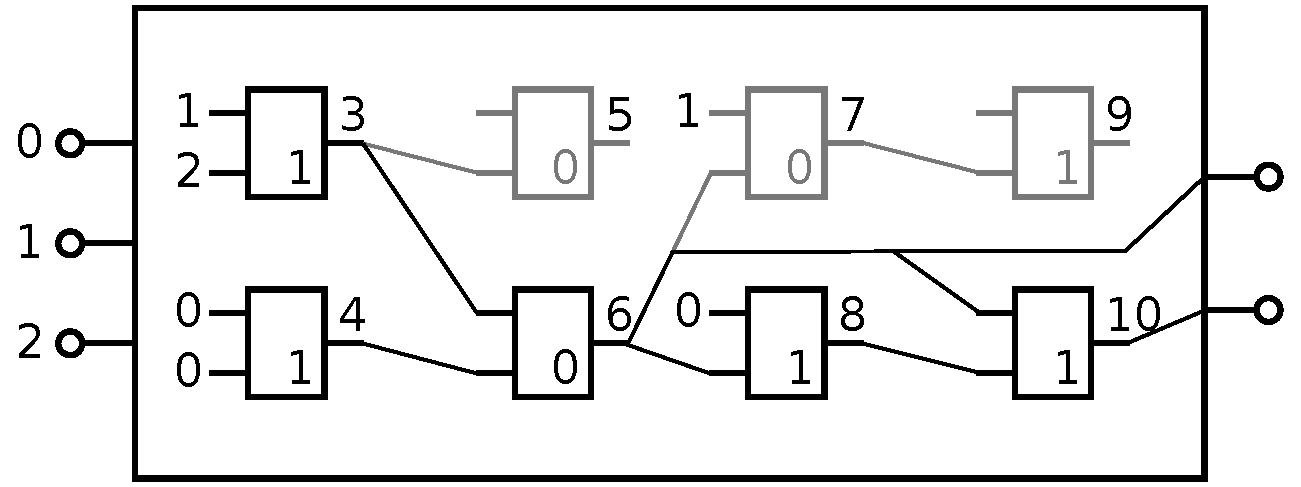
\includegraphics[width=0.8\linewidth]{images/cgp.pdf}
    \caption{Reprezentace programu v~kartézském genetickém programování.}
    \label{fig:CgpCircuit}
\end{figure}

CGP bylo úspěšně použito v~celé řadě úloh, jako je například symbolická regrese, klasifikace, návrh kombinačních obvodů nebo návrh obrazových filtrů. V~případě obrazových filtrů je na vstup kartézského programu přivedeno zvolené okolí zpracovávaného pixelu a výstupem je filtro\-va\-ný pixel. Jako fitness funkce se často používá špičková hodnota poměru signál/šum v~decibelech (Peak Signal to Noise Ratio, PSNR):

\begin{equation}
    \label{eq:PSNR}
    \mathit{PSNR} = 10 \log_{10} \frac{255^2}{\frac{1}{MN} \sum\limits_{i,j} \left( v\left( i, j \right) - w\left( i, j \right)  \right)^2 }
\end{equation}

\noindent{}kde $M$ a $N$ označují rozměry obrázku, $v$ filtrovaný a $w$ cílový (nepoškozený) obrázek \cite{ZelenaIF}.

Pro výpočet fitness kandidátního filtru musíme zpracovat celý obrázek, přičemž každý pixel lze považovat za jeden případ fitness. Protože i pro po\-měrně malé obrázky jich je několik tisíc, je výpočet fitness časově velmi náročný.

Tento problém se dá řešit pomocí koevolučního algoritmu. Při koevoluci se souběžně vyvíjí několik různých populací, které mezi sebou interagují prostřednictvím fitness funkcí. Fitness jedince závisí kromě jeho fenotypu také i na jedincích z~okolních populací. V~případě koevoluce s~prediktory fitness existují dvě populace a archiv, do kterého jsou vkládána nej\-lep\-ší nalezená kandidátní řešení (viz schéma na obrázku~\ref{fig:CoevolutionScheme}). Ta jsou vyvíjena pomocí CGP a jako fitness funkce slouží predikovaná fitness $f_{\mathit{predicted}}$, která je určená pomocí nej\-lep\-šího nalezeného prediktoru. Po vložení nového jedince do archivu se vypočítá i jeho skutečná fitness $f_{\mathit{exact}}$, pomocí které se ohodnocují prediktory.

Ve druhé populaci se pomocí genetického algoritmu vyvíjí prediktory fitness, což jsou pod\-mno\-žiny mno\-žiny případů fitness (pixelů trénovacího obrázku). Jejich chromozomy jsou vek\-tory ukazatelů do trénovací množiny o~konstantní délce. Potomci jsou tvořeni pomocí křížení a mutace, kvůli zachování diverzity populace je ně\-ko\-lik potomků vytvářeno zcela náhodně. Využívá se i eli\-tis\-mus, kdy několik nejlepších jedinců rodičovské populace přechází do populace potomků. Fitness prediktoru je určena jako střední absolutní odchylka skutečné a predikované fitness všech programů v~archivu:

\begin{equation}
    \label{eq:fitnessPredictor}
    f \left( p \right) = \frac{1}{u} \sum\limits_{i=1}^{u} \left| f_{\mathit{exact}} \left( s\left( i \right) \right) - f_{\mathit{predicted}} \left( s\left( i \right) \right) \right|
\end{equation}

\noindent{}kde $p$ označuje prediktor a $s$ archiv programů, který obsahuje $u$ jedinců. Prediktor s~nejnižší odchylkou je pak použit pro ohodnocování kandidátních filtrů.

Po spuštění programu jsou náhodně vytvořeny po\-čá\-teč\-ní populace filtrů a prediktorů fitness. Poté je vypočtena skutečná fitness filtrů a nejlepší jedinec je umís\-těn do archivu. Pomocí něj jsou následně ohod\-no\-ceny prediktory fitness a je určen nejlepší z~nich, který bude zpočátku sloužit pro výpočet predikované fitness. Po této inicializaci archivů pokračuje běh programu ve dvou vláknech, ve kterých probíhá evoluce jed\-not\-li\-vých populací \cite{SikuPPSN}.

\begin{figure*}[t]
    \centering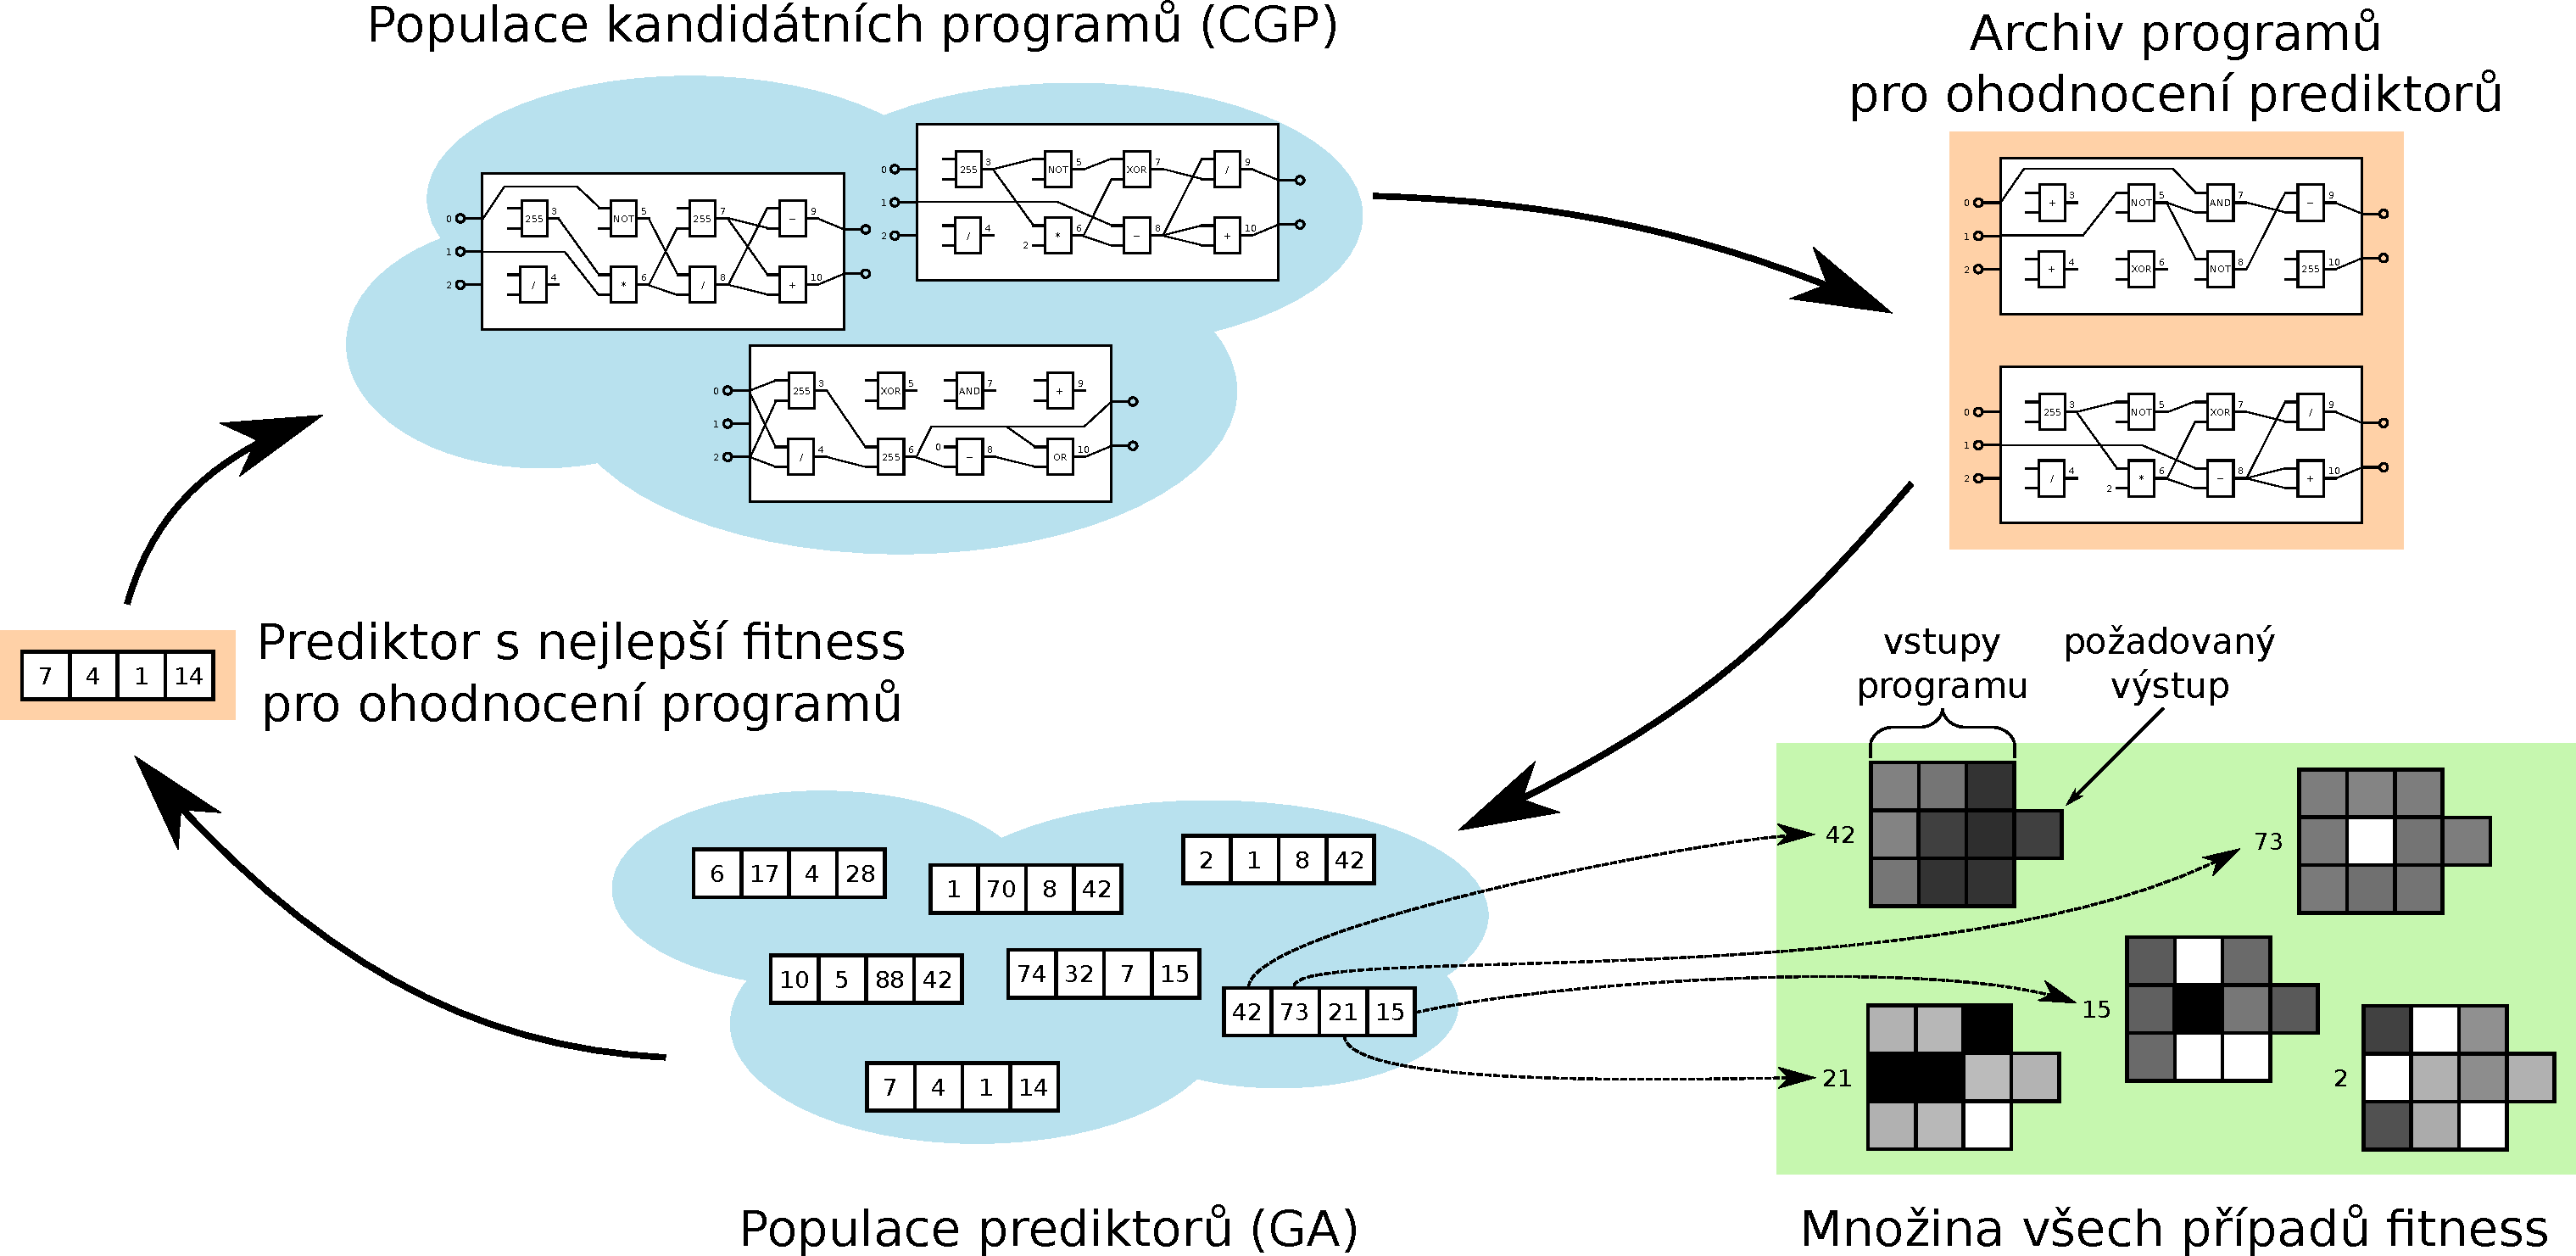
\includegraphics[width=0.8\linewidth]{images/coevolution-if.pdf}
    \caption{Schéma koevoluce CGP a prediktorů fitness.}
    \label{fig:CoevolutionScheme}
\end{figure*}



%--------------------------------------------------------
%--------------------------------------------------------
%--------------------------------------------------------
%--------------------------------------------------------
\section{Adaptivní velikost prediktorů fitness}
\label{sec:AdaptiveSize}

Nevýhodou koevolučního přístupu je nutnost předem stanovit velikost prediktoru, přičemž pro různé úlohy je výhodnější použít jinou velikost. Před použitím koevolučního CGP pro řešení nového problému je pak někdy nutné provést celou řadu časově náročných experimentů, jejichž cílem je určit nejvýhodnější velikost prediktoru. Cílem této práce je navrhnout, implementovat a experimentálně vyhodnotit algoritmus pro návrh obrazových filtrů, který využívá koevoluci s~přímo kódovanými prediktory, jejichž velikost se adaptuje v~průběhu evoluce na obtížnost úlohy.

\subsection{Kódování prediktorů fitness}

Při evoluci se souběžným učením mají jedinci tzv. plas\-tický fenotyp. Jako plasticita se označuje schopnost jedince přizpůsobit se pomocí učení na své prostředí~-- jeho fenotyp pak nezáleží jen na genotypu, ale také na okolních vlivech \cite{EllefsenBalancing}. U~prediktorů s~plastickým fenotypem se může jejich velikost adaptovat na složitost řešeného problému a stav evoluce. Plasticita je dosažena tím, že fenotyp prediktoru netvoří všechny ukazatele obsažené v~genotypu, ale pouze jejich část.

Fenotyp se z~genotypu tvoří postupným čtením genů od zvolené pozice. Pokud hodnota (ukazatel do množiny případů fitness) právě čteného genu není obsažena ve fenotypu, je do něj vložena, v~opačném případě se gen ignoruje. Poté je přečten další gen a proces se opakuje. Během tvorby fenotypu nejsou čteny úplně všechny geny -- jejich počet je určen proměnnou \emph{UsedGenes}, která je součástí prostředí a v~průběhu evoluce se mění. Pokud je při čtení dosaženo konce genotypu, ale nebyl ještě přečten potřebný počet genů, pokračuje se od jeho začátku. Příklad tvorby fenotypu při použití šesti genů z~devíti ukazuje obrázek \ref{fig:PhenotypeContruction}. Počátek čtení určuje zvláštní gen, který je modifikován speciálním mutačním operátorem. Ten k~současné hod\-notě genu přičítá malé náhodné číslo generované s~normálním rozdělením.

\begin{figure}[b]
    \centering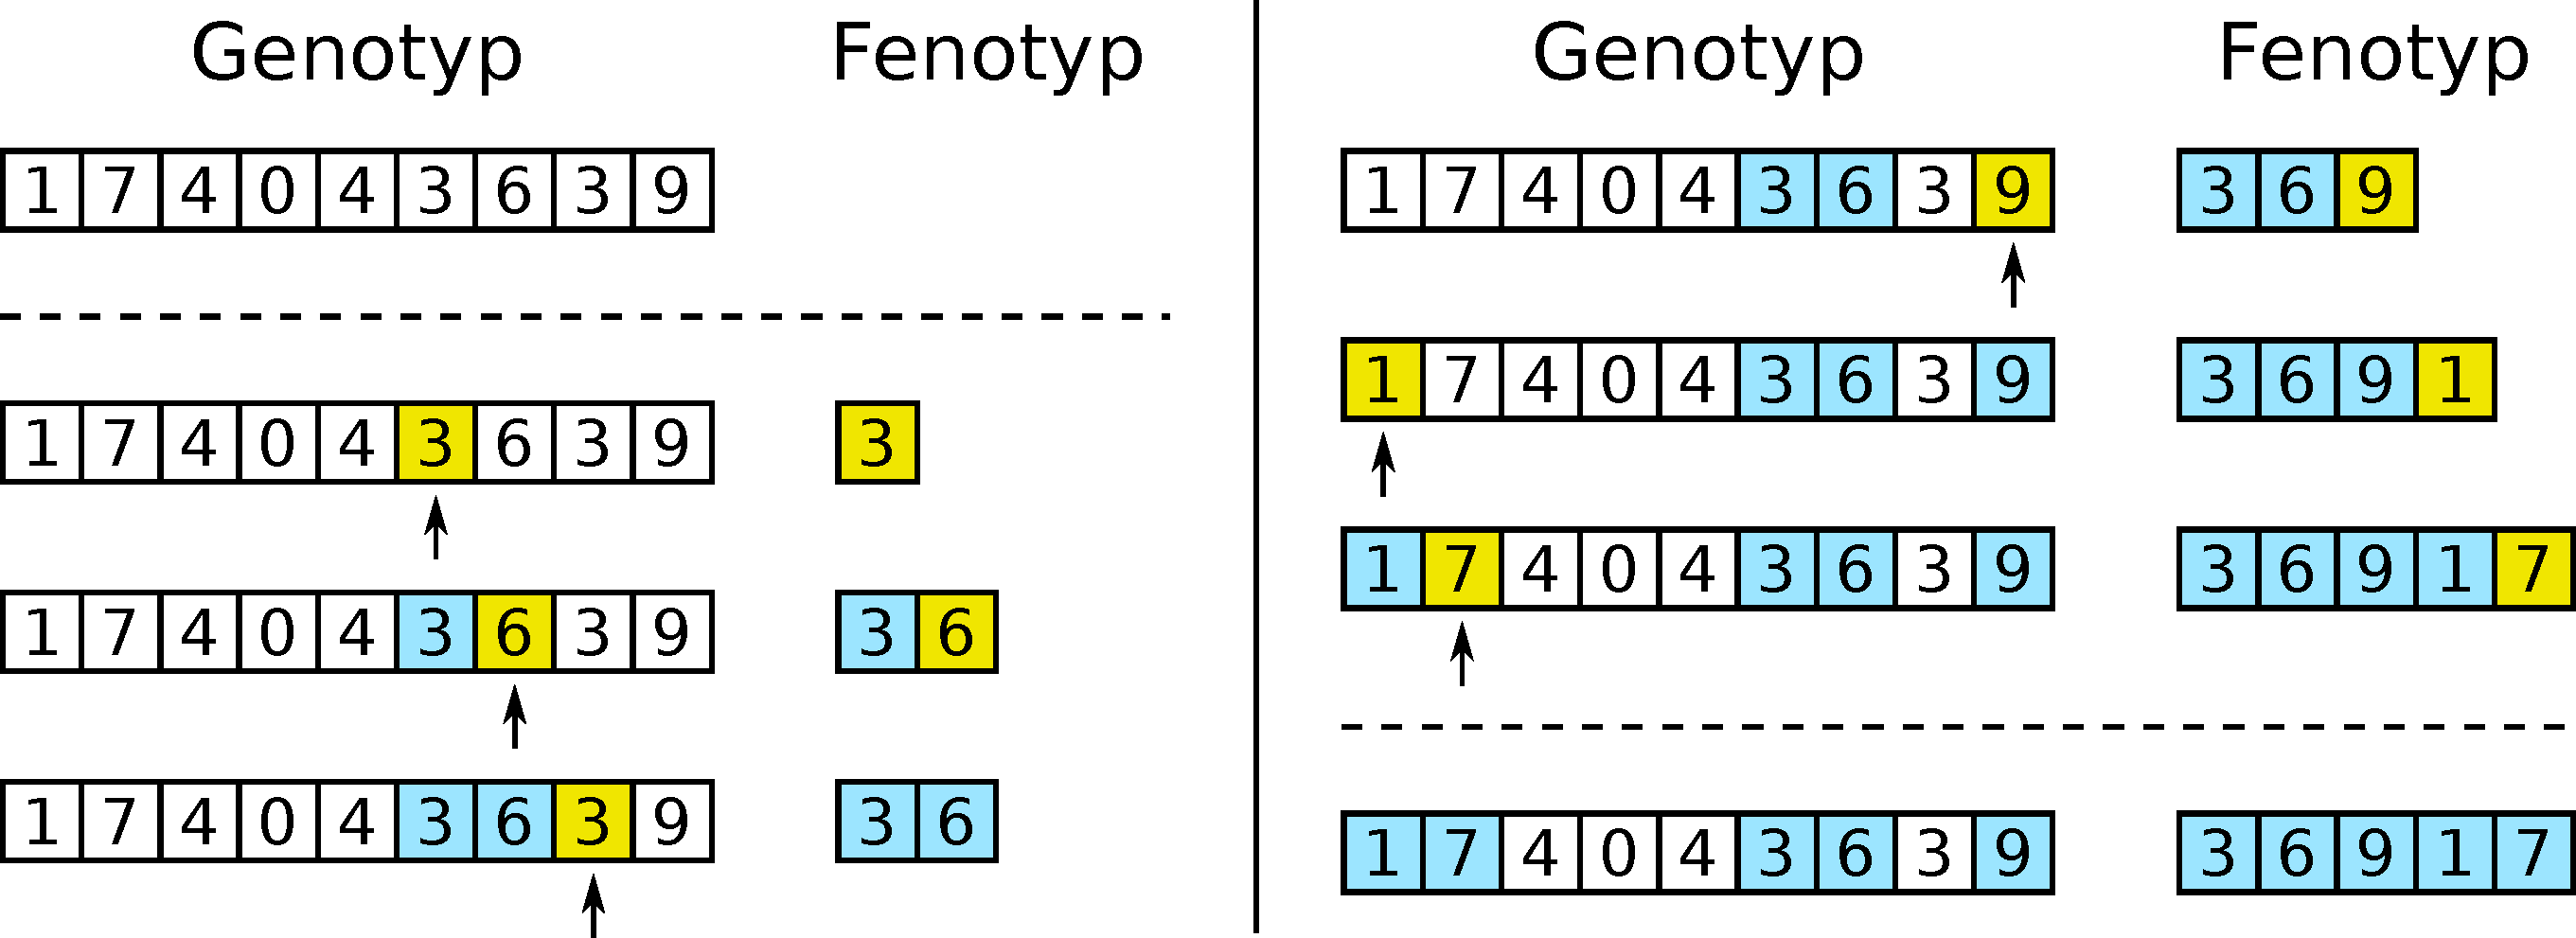
\includegraphics[width=\linewidth]{images/phenotype2.pdf}
    \caption{Postup konstrukce fenotypu prediktoru. Šipka označuje právě přečtený gen.}
    \label{fig:PhenotypeContruction}
\end{figure}

\subsection{Adaptace velikosti prediktorů}

Adaptace velikosti prediktoru probíhá na základě sledování rychlosti vývoje skutečné fitness kan\-di\-dát\-ních ře\-šení. Lze očekávat, že jejich populace prochází ob\-do\-bími, kdy je celková schopnost adaptace vyšší (a~fitness populace stoupá) a obdobími, kdy se adaptovat příliš nedokáže (a fitness se nemění). Důležitý je i~směr změny fitness, protože je pro ohodnocení je\-dinců v~CGP používána predikovaná fitness a skutečná fitness nejlepšího jedince může i klesat. Rychlost je možné například určit jako podíl změny fitness nej\-lep\-šího jedince v~populaci a počtu generací, které uběhly od minulé změny:

\begin{equation}
    \label{eq:velocity}
    v~= \frac{\Delta{}f_{\mathit{exact}}}{\Delta{}G}
\end{equation}

U~příliš krátkých prediktorů (v~extrémním případě to může být i jen jeden případ fitness) hrozí, že se velmi dobře adaptují na kandidátní řešení uložená v~archivu a predikce u~jiných filtrů bude velmi nepřesná. Proto se sleduje i nepřesnost predikce a pokud překročí stanovenou mez, prediktory se prodlouží. Nepřesnost prediktoru je vypočtena při každé změně rodiče v~CGP jako poměr mezi predikovanou a skutečnou hodnotou fitness nejlepšího filtru v~populaci:

\begin{equation}
    \mathit{I} = \frac{f_{\mathit{predicted}}}{f_{\mathit{exact}}}
\end{equation}

Vždy po vložení kandidátního programu do ar\-chivu je zvolen koeficient, kterým se vynásobí sou\-časná hodnota proměnné \emph{UsedGenes}, čímž se změní velikost fenotypů prediktorů. Pravidla pro určení tohoto koeficientu jsou následující: 1)~Pokud je nepřesnost pre\-dikce příliš vysoká, pre\-dik\-to\-ry se prodlouží. 2)~Pokud se fitness nemění ($v \approx 0$), evoluce prav\-dě\-po\-dob\-ně uvázla v~lokálním op\-ti\-mu, pre\-dik\-tory se zkrátí, což může pomoci se z~tohoto op\-ti\-ma po\-su\-nout dále. 3)~Pokud fitness klesá ($v < 0$), evoluce prav\-dě\-po\-dobně opouští lokální optimum a mírné zkrácení prediktoru může pomoci postup urychlit. 4)~Pokud fitness roste ($v > 0$), prediktory se prodlouží a tím se zpřesní predikce. Rozlišuje se mezi \uv{pomalým} a \uv{rychlým} růstem.


%--------------------------------------------------------
%--------------------------------------------------------
%--------------------------------------------------------
%--------------------------------------------------------
\section{Implementace}
\label{sec:Implementation}

Kvůli velkému množství plánovaných experimentů byl kladen důraz především na co nejrychlejší běh programu. Implementován byl proto v~jazyce C, ve kterém lze snadno pracovat i s~assemblerem a rozšiřujícími instrukčními sadami procesoru.

Paralelizace je řešena pomocí direktiv překladače definovaných ve standardu OpenMP\footnote{\url{http://openmp.org/}} pro paralelní programování se sdílenou pamětí. Rozdělení do paralelních oblastí znázorňuje obrázek~\ref{fig:ParallelSections}. Při koevoluci je program rozdělen do dvou paralelních sekcí, ve kterých se vyvíjí jednotlivé populace. Ve sdílené paměti se nachází především nejlepší prediktor a archiv kandidátních programů. Paralelní sekce populací se navíc dělí na další vlákna při ohodnocování populací a při tvorbě potomků tak, že jsou jedinci zpracovávání paralelně.

\begin{figure}[htb]
    \centering
    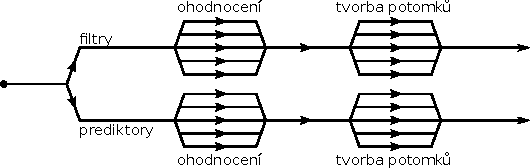
\includegraphics[width=0.9\linewidth]{images/openmp.pdf}
    \caption{Schéma paralelizace koevoluce.}
    \label{fig:ParallelSections}
\end{figure}

Největší důraz byl kladen na optimalizaci rychlosti výpočtu výstupních hodnot kandidátních programů, což je časově nejnáročnější část výpočtu. Ta je imple\-men\-to\-vána třemi způsoby. V~nejjednodušším z~nich se každý výstupní pixel počítá zvlášť a pro zpra\-co\-vání celého obrázku o~rozměrech $256\times256$~pixelů je třeba 65~536 průchodů filtrem. Ve druhém případě se využívá instrukční sady SSE2, které přináší vek\-to\-rové instrukce nad 128bitovými registry. Díky tomu lze zpracovat 16~pixelů najednou. Nejrychlejší im\-ple\-men\-tace je založená na prozatím nejnovější instrukční sadě AVX2\footnote{Poprvé představena v~procesorech Intel Haswell v~roce 2013.}, ve které jsou všechny instrukce SSE rozšířeny o~podporu 256bitových registrů a lze tak počítat hodnoty 32~pixelů zároveň. Pro zpracování zmíněného obrázku pak stačí jen 2~048 průchodů filtrem.

Bohužel nelze využít starší a rozšířenější instrukční sadu AVX, protože neobsahuje instrukce pro 256bitové vektory celých čísel. V~budoucnu je možné program rozšířit o~implementaci s~512bitovými instrukcemi z~připravované instrukční sady AVX-512\footnote{První procesory s~podporou AVX-512 se objeví v~roce 2015.}.

Vektorizace výpočtu byla implementována pomocí tzv. intrinsic funkcí. Ty jsou překladačem přeloženy na konkrétní instrukci, například volání intrinsic funkce \texttt{\_mm\_add\_epi8} se přeloží jako instrukce \texttt{PADDB}.

Aby byl výpočet pomocí vektorových in\-strukcí efektivní, je potřeba upravit strukturu dat v~paměti. U~sériového výpočtu je výhodné trénovací data ukládat jako jedno pole všech devítiokolí. U~výpočtu pomocí SSE2 nebo AVX2 je ale třeba do registrů zko\-pí\-ro\-vat vektor 16 či 32 hodnot ze stejné pozice v~devítiokolí -- zde je lepší mít trénovací data uložena jako strukturu polí, z~nichž každé obsahuje pixely z~jedné pozice devítiokolí, resp. požadované výstupy programu.

Při ohodnocování kandidátních filtrů pomocí pre\-dik\-toru jsou vstupní hodnoty náhodně rozmístěny v~pa\-měti. Proto se pro každý nový prediktor a po změně fenotypu prediktoru nejprve zkopírují vstupní data do pomocných polí tak, aby byly vybrané případy fitness bezprostředně za sebou. Struktura trénovacích dat a ukázka takto připraveného prediktoru je na obrázku \ref{fig:SimdDataStructure}.


\begin{figure}[htb]
    \centering
    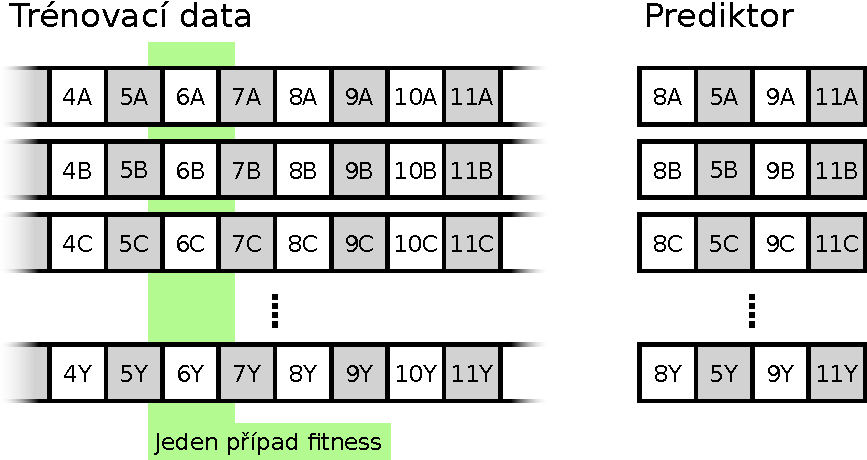
\includegraphics[width=0.82\linewidth]{images/simd4.pdf}
    \caption{Struktura trénovacích dat a prediktoru s~fenotypem \emph{$\left<8, 5, 9, 11\right>$} pro výpočet instrukcemi SSE2/AVX2. Písmeno Y označuje požadovaný výstup, ostatní písmena pozice v~devítiokolí.}
    \label{fig:SimdDataStructure}
\end{figure}

Vektorová implementace navíc využívá toho, že v~experimentech měla mřížka CGP vždy 4 řádky a \mbox{$l$-back} byl roven jedné. Aby se zmenšil počet přístupů do paměti, neukládají se výstupy funkčních bloků z~předchozího sloupce do paměti, ale jsou pro ně vyhrazeny čtyři registry SSE/AVX. Další čtyři registry slouží pro výstupy bloků v~právě počítaném sloupci.

Přeložený program obsahuje všechny tři implementace. Která z~nich se použije při výpočtu, závisí na tom, jaké instrukční sady podporuje počítač, na kterém je program spuštěn. To se zjišťuje pomocí instrukce \texttt{CPUID}. Pokud se používají instrukce ze sady SSE2, je k~dosažení stejného počtu generací CGP bez koevoluce potřeba přibližně desetina času oproti základní implementaci (pouze s~OpenMP), v~případě AVX2 je zrychlení zhruba šest\-nác\-ti\-ná\-sobné.

%--------------------------------------------------------
%--------------------------------------------------------
%--------------------------------------------------------
%--------------------------------------------------------
\section{Experimentální vyhodnocení}
\label{sec:Experimental}

Navržený algoritmus byl experimentálně ověřen na úloze návrhu obrazových filtrů. Cílem je nalézt vhodný filtr pro rekonstrukci obrázků poškozených impulzním šumem. U~tohoto typu šumu mají poškozené pixely náhodnou hodnotu. Při experimentování se pra\-co\-valo také s~šumem typu sůl a pepř, u~kterého mají poškozené pixely buď minimální nebo maximální možnou hodnotu. V~obou případech mohou být příčinou vadné body ve snímači v~kameře, nefunkční paměťové buňky nebo chyby při přenosu dat. Tyto typy šumu jsou charakterizovány svou in\-ten\-zi\-tou -- poměrným poč\-tem poškozených pixelů.

\subsection{Nastavení experimentů}

Nastavení kartézského genetického programování a genetického algoritmu vychází z~článku \cite{SikuPPSN}. Mřížka CGP má velikost $8 \times 4$, programy mají 9 vstupů (devíti\-okolí zpracovávaného pixelu) a 1 výstup (nová hodnota pixelu), parametr $l$-back je roven jedné. V~populaci je 8~jedinců, potomci jsou tvořeni mutací 1 až 5 genů.

U~prediktorů fitness se v~populaci vyvíjí 32 jedinců. Novou generaci tvoří 8 nejlepších jedinců, 16 jedinců vzniklých jednobodovým křížením a mutací až 5\,\% genů a 8 náhodných jedinců.

Parametry pro adaptaci velikost prediktorů byly určeny experimentálně. Celkem bylo spuštěno přes 170~000 nezávislých běhů programu, na jejichž základě byly zvoleny parametry pravidel změny velikosti uvedené v~tabulce \ref{table:rules}. Počáteční velikost prediktorů (hodnota \textit{UsedGenes}) je 3\,\% případů fitness, minimální a maximální velikost je bez omezení. Při tvorbě fenotypu prediktoru se ge\-notyp čte vždy od jeho počátku.

Trénovací data pochází z~webu ImageProcessingPlace.com, kde se nacházejí databáze obrázků po\-uží\-vaných komunitou zabývající se zpracováním obrazu.

\begin{table}[hbt]
    \vskip6pt
    \caption{Pravidla pro změnu proměnné \textit{UsedGenes}. Při splnění více podmínek se uplatní první z~nich.}
    \label{table:rules}
    \centering
    \small
    \renewcommand{\arraystretch}{1.1}
    \begin{tabular}{llll}
        \toprule
        \multicolumn{2}{l}{podmínka}      &  nová hodnota \textit{UsedGenes}  \\
        \midrule
        1. &  $I > 1,2$                   &  $\mathit{UsedGenes} \cdot 2    $     \\
        2. &  $\left|v\right| \leq 0,001$ &  $\mathit{UsedGenes} \cdot 0,93 $  \\
        3. &  $v < 0$                     &  $\mathit{UsedGenes} \cdot 0,96 $  \\
        4. &  $0 < v~\leq 0,1$            &  $\mathit{UsedGenes} \cdot 1,07 $  \\
        5. &  $v > 0,1$                   &  beze změny             \\
        \bottomrule
    \end{tabular}
\end{table}

Dosažené výsledky byly porovnány se standardním CGP a také s~koevolučním CGP s~prediktory fitness o~délce 0,5\,\%, 1\,\%, 2\,\%, 3\,\%, 4\,\%, 5\,\%, 10\,\%, 15\,\%, 20\,\% a 25\,\%. Výsledky všech experimentů jsou souhrnem ze 100 nezávislých běhů pro každé nastavení po uplynutí 30~000 generací CGP.

Výpočty probíhaly na superpočítači Anselm, \mbox{jehož} každý výpočetní uzel obsahuje dva osmijádrové procesory Intel Xeon E5-2665 (2,4 až 3,1\,GHz s~technologií Turbo Boost) nebo Intel Xeon E5-2470 (2,3 až 3,1\,GHz s~technologií Turbo Boost) a alespoň 64 GB operační paměti. Tyto procesory mají starší architekturu Sandy Bridge a nepodporují instrukční sadu AVX2.

\subsection{Schopnost adaptace velikosti prediktoru}

Ukazuje se, že nezávisle na jejím počátečním nastavení, konverguje velikost prediktoru ke stejné hodnotě, která se liší úlohu od úlohy. Příklad průběhu velikosti u~5\% šumu typu sůl a pepř je na obrázku~\ref{fig:InitialSize}. Také kvalita nalezených filtrů je srovnatelná bez ohledu na nastavení. Je tedy vhodné začínat s~men\-šími pre\-dik\-tory, protože výpočet $f_\mathit{predicted}$ je pak rychlejší.

% \begin{figure}[h]
%     \centering
%     \subfloat[5\% šum sůl a pepř]{
%         \centering
%             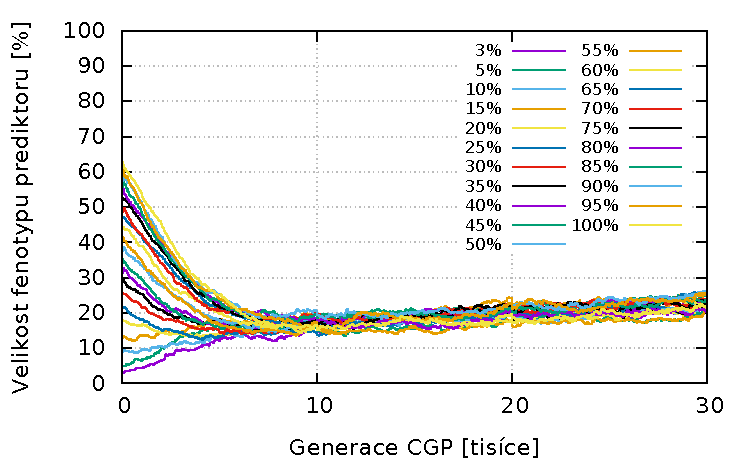
\includegraphics[width=0.9\linewidth]{images/initial-size-5-30kg.pdf}
%     }\\
%     \subfloat[50\% šum sůl a pepř]{
%         \centering
%             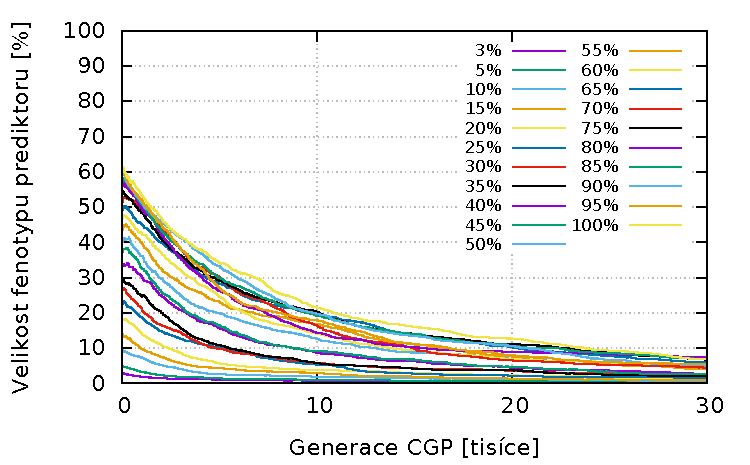
\includegraphics[width=0.9\linewidth]{images/initial-size-50-30kg.pdf}
%     }
%     \caption{Vývoj velikosti prediktorů fitness při různé počáteční velikosti.}
%     \label{fig:InitialSize}
% \end{figure}

\begin{figure}[htb]
    \centering
    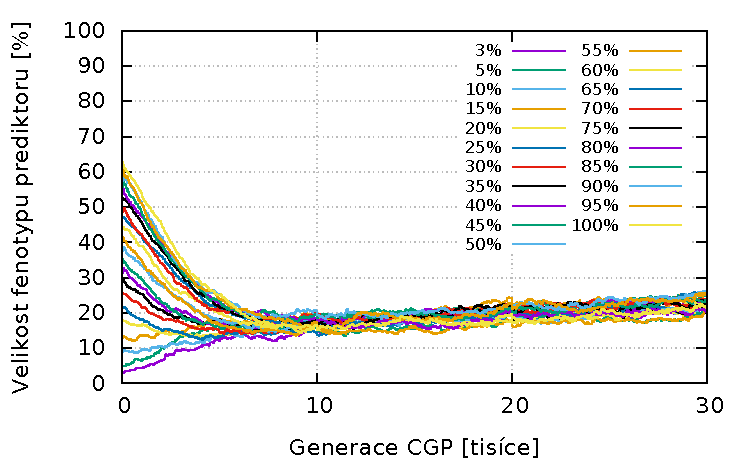
\includegraphics[width=0.9\linewidth]{images/initial-size-5-30kg.pdf}
    \caption{Vývoj velikosti prediktorů fitness při různé počáteční velikosti u~5\% šumu sůl a pepř.}
    \label{fig:InitialSize}
\end{figure}

\subsection{Kvalita filtrů a doba běhu}

Cílem experimentů bylo srovnání navrženého algoritmu CGP s~adaptivními prediktory fitness ($\mathit{FP_{ADAPT}}$) s~koevolučním CGP s~prediktory pevné délky ($\mathit{FP_{FIX}}$) a s~CGP bez koevoluce ($\mathit{CGP_{STD}}$) s~ohledem na kvalitu nalezených obrazových filtrů a na délku běhu evoluce. Experimenty byly provedeny na obrázcích se šumem o~intenzitě 10 až 80\,\% s~krokem po 10\,\%.

Jak je vidět na příkladu 10\% impulzního šumu na obrázku~\ref{fig:ImpulseBoxplot}, je kvalita filtrů nalezená pomocí $\mathit{FP_{ADAPT}}$ srovnatelná s~filtry získanými $\mathit{CGP_{STD}}$ a $\mathit{FP_{FIX}}$ s~pre\-dik\-tory o~velikosti 10\,\% a více. Co se týče potřebného času, je v~tomto případě $\mathit{FP_{ADAPT}}$ v~průměru 6,26krát rychlejší než $\mathit{CGP_{STD}}$. Také je srovnatelně rychlý jako při použití $\mathit{FP_{FIX}}$ s~3--5\% pre\-dik\-to\-rem, kdy ale mají výsledné filtry nižší kvalitu než u~$\mathit{FP_{ADAPT}}$.

Podobné výsledky byly dosaženy i pro jiné in\-ten\-zity šumu. Konkrétní hodnoty jsou uvedeny v~ta\-bulce~\ref{table:results} a některé testovací obrázky po zpracování nej\-lepším nalezeným filtrem jsou na obrázku \ref{fig:BestImages}. Ve všech pří\-pa\-dech je kvalita filtrů získaných pomocí $\mathit{FP_{ADAPT}}$ srovnatelná při kratší nebo přinejhorším podobné době běhu. V~průměru bylo dosaženo 8,39násobného zrychlení oproti $\mathit{CGP_{STD}}$.


\begin{figure}[ht]
    \centering
    \subfloat[Kvalita filtrů (červeně průměr PSNR všech filtrů)]{
        \centering
        \hskip12pt
        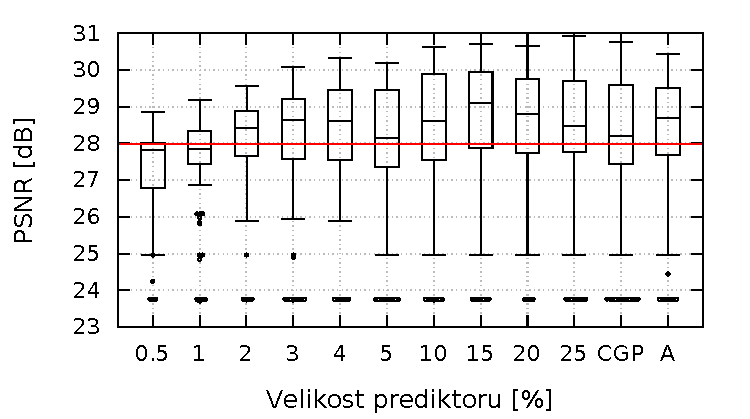
\includegraphics[width=0.86\linewidth]{images/impulse10-30kg-psnr-mean.pdf}
        \hskip12pt
    }\\
    \subfloat[Čas běhu (součet všech vláken)]{
        \centering
            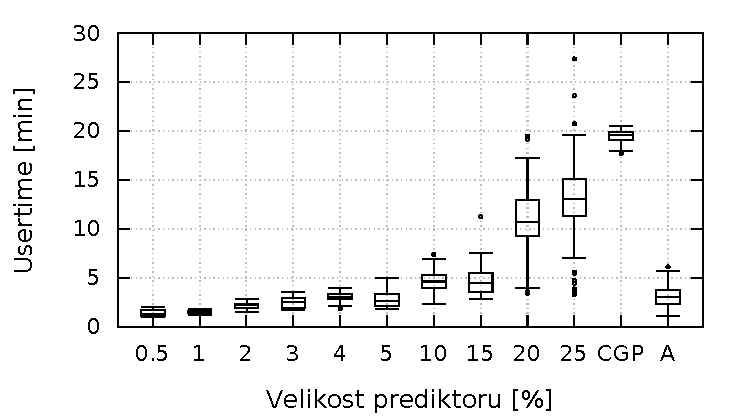
\includegraphics[width=0.86\linewidth]{images/impulse10-30kg-usertime.pdf}
    }
    \caption{Srovnání CGP, koevolučního CGP s~prediktory fitness různých velikostí a s~prediktory fitness s~adaptivní velikostí (A) pro 10\% impulzní šum po 30~000 generacích.}
    \label{fig:ImpulseBoxplot}
\end{figure}


\begin{figure*}[b!]
    \centering
    \newcommand{\size}{0.22}
    \subfloat[Obrázek 1 (20\% šum)]{
        \centering
            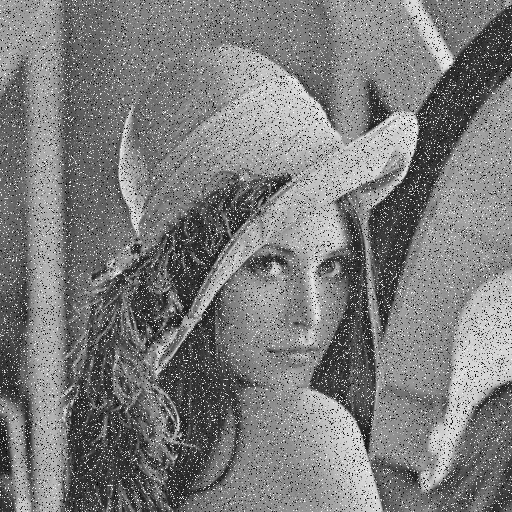
\includegraphics[width=\size\linewidth]{images/imp20}
    }\hfill
    \subfloat[Obrázek 2 (30\% šum)]{
        \centering
            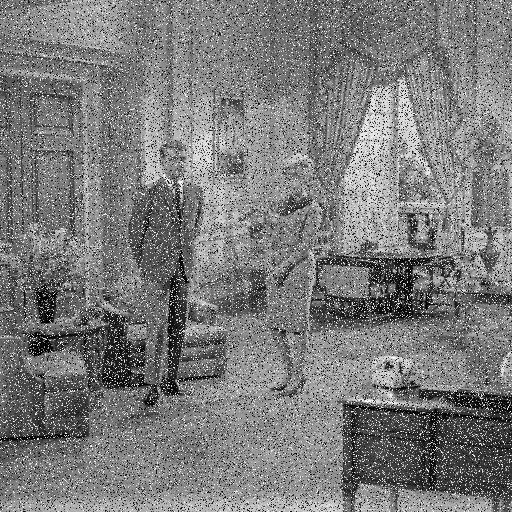
\includegraphics[width=\size\linewidth]{images/imp30}
    }\hfill
    \subfloat[Obrázek 3 (40\% šum)]{
        \centering
            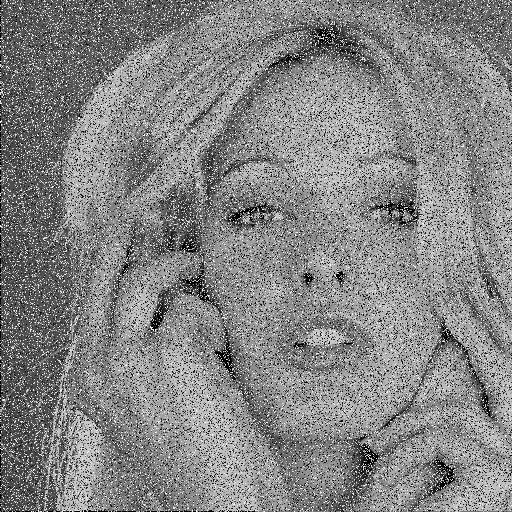
\includegraphics[width=\size\linewidth]{images/imp40}
    }\hfill
    \subfloat[Obrázek 4 (50\% šum)]{
        \centering
            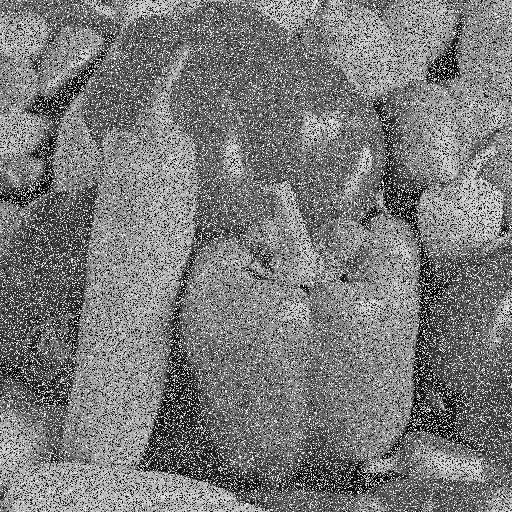
\includegraphics[width=\size\linewidth]{images/imp50}
    }\\
    \subfloat[Filtrovaný obrázek 1]{
        \centering
            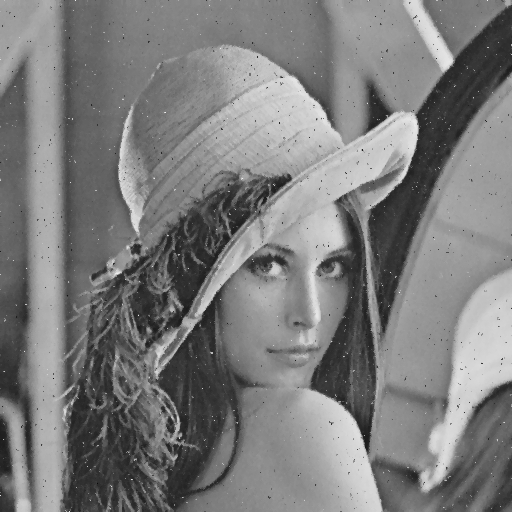
\includegraphics[width=\size\linewidth]{images/imp20filtered}
    }\hfill
    \subfloat[Filtrovaný obrázek 2]{
        \centering
            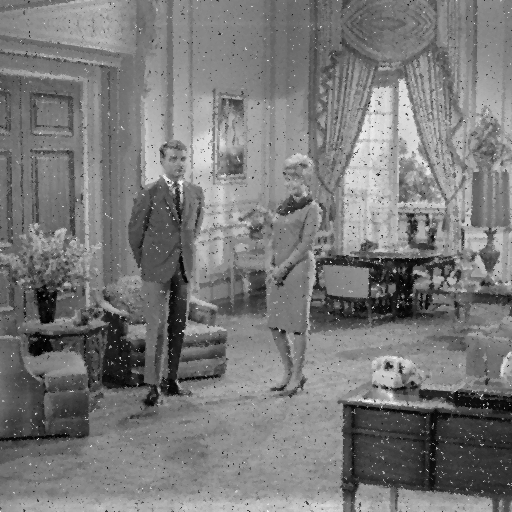
\includegraphics[width=\size\linewidth]{images/imp30filtered}
    }\hfill
    \subfloat[Filtrovaný obrázek 3]{
        \centering
            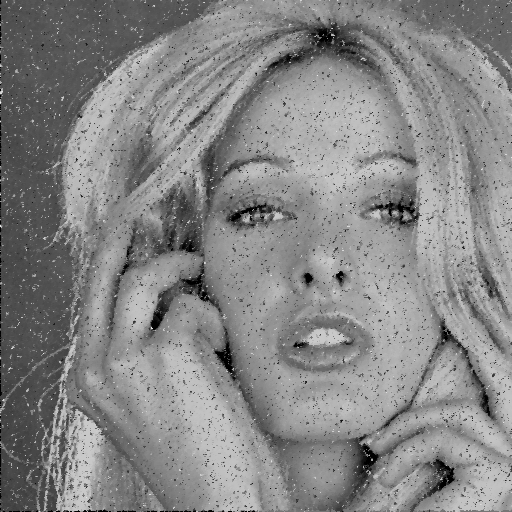
\includegraphics[width=\size\linewidth]{images/imp40filtered}
    }\hfill
    \subfloat[Filtrovaný obrázek 4]{
        \centering
            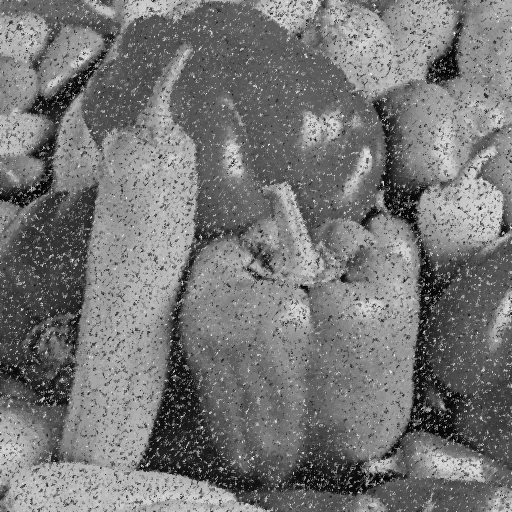
\includegraphics[width=\size\linewidth]{images/imp50filtered}
    }
    \caption{Testovací obrázky filtrované nejlepšími filtry (jeden krok filtrace) nalezenými pomocí koevoluce s~adaptivními prediktory fitness.}
    \label{fig:BestImages}
\end{figure*}



%--------------------------------------------------------
%--------------------------------------------------------
%--------------------------------------------------------
%--------------------------------------------------------
\section{Závěr}
\label{sec:Conclusions}

V~tomto článku byl představen nový způsob kódování prediktorů fitness v~koevolučním CGP, který umožňuje tvořit ze stejného genotypu různé fenotypy. Díky takto získaně plasticitě lze průběžně měnit jejich velikost a reagovat tak na průběh evoluce kandidátních řešení a na složitost řešeného problému. Z~provedených ex\-pe\-ri\-mentů na úloze návrhu obrazových filtrů vyplývá, že kvalita získaných filtrů se příliš neliší od výsledků koevoluce s~prediktory pevné délky a také od výsledků standardního CGP. Oproti standardnímu CGP bylo dosaženo v~průměru 8,39násobného zrychlení. Také odpadá nutnost časově náročného experimentálního hledání nejvýhodnější velikosti prediktorů pro danou úlohu, což je jedna z~nevýhod koevoluce.

V~dalším pokračování této práce bude představený koncept apli\-ko\-ván v~úloze návrhu složitých kombinačních obvodů.


\begin{table*}[t!]
\centering
    \caption{Srovnání standardního CGP, CGP s~koevolucí s~prediktory různých délek a s~prediktory s~adap\-tivní velikostí po 30~000 generacích. Řešenou úlohou je filtr pro impulzní šum různé intenzity. U~$\mathit{FP_{FIX}}$ byly testovány délky 0,5, 1, 2, 3, 4, 5, 10, 15, 20 a 25 procent, v~tabulce je jen výsledek s~nejlepším průměrným PSNR. U~$\mathit{FP_{ADAPT}}$ je uvedena průměrná délka prediktoru.}
    \label{table:results}
    \renewcommand{\arraystretch}{1}
    \scriptsize
        \hfill
        \begin{minipage}[t]{.48\textwidth}
            \centering
            \begin{tabular}{=c +l +c +c +c +c}
                \toprule

                \multirow{2}{1cm}{\centering{}Intenzita} & \multirow{2}{*}{} & \multirow{2}{*}{} &
                \multirow{2}{*}{$\mathit{CGP_{STD}}$} & \multirow{2}{*}{$\mathit{FP_{FIX}}$} & \multirow{2}{*}{$\mathit{FP_{ADAPT}}$} \\
                \\

                \midrule
                \multirow{8}{*}{10\,\%}
                & Prediktor [\%]    &&  --  &   15  &   7,59    \\
                \cmidrule{2-6}
                \rowstyle{\color{grayintable}}
                & \multirow{3}{*}{\color{black}PSNR\,[dB]}
                & Min.      &   23,76   &   23,76   &   23,76   \\
                && Průměr   &   27,91   &   28,61   &   28,20   \\  \rowstyle{\color{grayintable}}
                && Max.     &   30,75   &   30,72   &   30,43   \\
                \cmidrule{2-6}
                \rowstyle{\color{grayintable}}
                & \multirow{3}{*}{\color{black}Čas\,[min]}
                & Min.      &   17,73   &   2,85    &   1,10    \\
                && Průměr   &   19,46   &   4,72    &   3,11    \\  \rowstyle{\color{grayintable}}
                && Max.     &   20,55   &   11,28   &   6,15    \\

                \midrule
                \multirow{8}{*}{20\,\%}
                & Prediktor [\%]    &&  --  &   25  &   4,08 \\
                \cmidrule{2-6}
                \rowstyle{\color{grayintable}}
                & \multirow{3}{*}{\color{black}PSNR\,[dB]}
                & Min.      &   20,91   &   20,91   &   20,91   \\
                && Průměr   &   24,80   &   25,18   &   24,82   \\  \rowstyle{\color{grayintable}}
                && Max.     &   27,31   &   27,57   &   27,07   \\
                \cmidrule{2-6}
                \rowstyle{\color{grayintable}}
                & \multirow{3}{*}{\color{black}Čas\,[min]}
                & Min.      &   16,97   &   3,67    &   1,18    \\
                && Průměr   &   19,42   &   9,30    &   2,66    \\  \rowstyle{\color{grayintable}}
                && Max.     &   20,73   &   24,80   &   4,00    \\

                \midrule
                \multirow{8}{*}{30\,\%}
                & Prediktor [\%]    &&  --  &   15  &   2,94 \\
                \cmidrule{2-6}
                \rowstyle{\color{grayintable}}
                & \multirow{3}{*}{\color{black}PSNR\,[dB]}
                & Min.      &   19,11   &   19,11   &   18,98   \\
                && Průměr   &   22,37   &   22,56   &   22,35   \\  \rowstyle{\color{grayintable}}
                && Max.     &   24,54   &   24,42   &   24,15   \\
                \cmidrule{2-6}
                \rowstyle{\color{grayintable}}
                & \multirow{3}{*}{\color{black}Čas\,[min]}
                & Min.      &   14,83   &   5,28    &   1,12    \\
                && Průměr   &   19,33   &   9,49    &   2,49    \\  \rowstyle{\color{grayintable}}
                && Max.     &   20,72   &   23,78   &   4,22    \\

                \midrule
                \multirow{8}{*}{40\,\%}
                & Prediktor [\%]    &&  --  &   15  &   1,65 \\
                \cmidrule{2-6}
                \rowstyle{\color{grayintable}}
                & \multirow{3}{*}{\color{black}PSNR\,[dB]}
                & Min.      &   17,66   &   17,38   &   17,22   \\
                && Průměr   &   20,11   &   20,21   &   19,79   \\  \rowstyle{\color{grayintable}}
                && Max.     &   22,25   &   21,81   &   21,53   \\
                \cmidrule{2-6}
                \rowstyle{\color{grayintable}}
                & \multirow{3}{*}{\color{black}Čas\,[min]}
                & Min.      &   17,43   &   2,58    &   1,02    \\
                && Průměr   &   19,31   &   6,53    &   2,45    \\  \rowstyle{\color{grayintable}}
                && Max.     &   20,62   &   22,32   &   3,80    \\

                \bottomrule
            \end{tabular}
        \end{minipage}
        \hfill
        \begin{minipage}[t]{.48\textwidth}
            \centering
            \begin{tabular}{=c +l +c +c +c +c}
                \toprule

                \multirow{2}{1cm}{\centering{}Intenzita} & \multirow{2}{*}{} & \multirow{2}{*}{} &
                \multirow{2}{*}{$\mathit{CGP_{STD}}$} & \multirow{2}{*}{$\mathit{FP_{FIX}}$} & \multirow{2}{*}{$\mathit{FP_{ADAPT}}$} \\
                \\

                \midrule
                \multirow{8}{*}{50\,\%}
                & Prediktor [\%]    &&  --  &   4   &   1,22 \\
                \cmidrule{2-6}
                \rowstyle{\color{grayintable}}
                & \multirow{3}{*}{\color{black}PSNR\,[dB]}
                & Min.      &   16,49   &   16,48   &   15,75   \\
                && Průměr   &   18,20   &   18,35   &   18,04   \\  \rowstyle{\color{grayintable}}
                && Max.     &   19,40   &   19,55   &   19,02   \\
                \cmidrule{2-6}
                \rowstyle{\color{grayintable}}
                & \multirow{3}{*}{\color{black}Čas\,[min]}
                & Min.      &   18,00   &   2,13    &   1,53    \\
                && Průměr   &   19,49   &   4,54    &   2,64    \\  \rowstyle{\color{grayintable}}
                && Max.     &   20,62   &   7,53    &   4,12    \\

                \midrule
                \multirow{8}{*}{60\,\%}
                & Prediktor [\%]    &&  --  &   20   &   0,80 \\
                \cmidrule{2-6}
                \rowstyle{\color{grayintable}}
                & \multirow{3}{*}{\color{black}PSNR\,[dB]}
                & Min.      &   15,08   &   15,48   &   15,47   \\
                && Průměr   &   16,71   &   16,81   &   16,52   \\  \rowstyle{\color{grayintable}}
                && Max.     &   17,45   &   17,48   &   17,04   \\
                \cmidrule{2-6}
                \rowstyle{\color{grayintable}}
                & \multirow{3}{*}{\color{black}Čas\,[min]}
                & Min.      &   17,50   &   5,00    &   0,85    \\
                && Průměr   &   19,44   &   11,98   &   2,92    \\  \rowstyle{\color{grayintable}}
                && Max.     &   20,43   &   47,73   &   5,27    \\

                \midrule
                \multirow{8}{*}{70\,\%}
                & Prediktor [\%]    &&  --  &   20  &   0,62    \\
                \cmidrule{2-6}
                \rowstyle{\color{grayintable}}
                & \multirow{3}{*}{\color{black}PSNR\,[dB]}
                & Min.      &   14,66   &   14,64   &   14,52   \\
                && Průměr   &   15,64   &   15,65   &   15,43   \\  \rowstyle{\color{grayintable}}
                && Max.     &   16,08   &   16,04   &   15,86   \\
                \cmidrule{2-6}
                \rowstyle{\color{grayintable}}
                & \multirow{3}{*}{\color{black}Čas\,[min]}
                & Min.      &   17,00   &   5,28    &   0,85    \\
                && Průměr   &   19,41   &   18,22   &   3,01    \\  \rowstyle{\color{grayintable}}
                && Max.     &   20,43   &   56,27   &   4,98    \\

                \midrule
                \multirow{8}{*}{80\,\%}
                & Prediktor [\%]    &&  --  &   10  &   0,65    \\
                \cmidrule{2-6}
                \rowstyle{\color{grayintable}}
                & \multirow{3}{*}{\color{black}PSNR\,[dB]}
                & Min.      &   14,52   &   14,52   &   14,52   \\
                && Průměr   &   14,85   &   14,85   &   14,70   \\  \rowstyle{\color{grayintable}}
                && Max.     &   15,11   &   15,15   &   15,06   \\
                \cmidrule{2-6}
                \rowstyle{\color{grayintable}}
                & \multirow{3}{*}{\color{black}Čas\,[min]}
                & Min.      &   16,52   &   4,72    &   0,80    \\
                && Průměr   &   19,41   &   11,24   &   1,96    \\  \rowstyle{\color{grayintable}}
                && Max.     &   20,57   &   24,85   &   3,40    \\

                \bottomrule
            \end{tabular}
        \end{minipage}
        \hfill
\end{table*}


%--------------------------------------------------------
%--------------------------------------------------------
%--------------------------------------------------------
%--------------------------------------------------------
\section*{Poděkování}
\label{sec:Acknowledgements}

Děkuji Ing. Michaele Šikulové nejen za cenné rady, náměty a nápady, ale především za její trpělivost a za veškerý čas, který mi věnovala v~souvislosti s~řešením této a diplomové práce.

Tato práce byla podporována projekty Vysokého učení technického v~Brně FIT-S-14-2297 a Centra excelence IT4Innovations CZ.1.05/1.1.00/02.0070.

%--------------------------------------------------------
%--------------------------------------------------------
%--------------------------------------------------------
%	REFERENCE LIST
%--------------------------------------------------------
%--------------------------------------------------------
\phantomsection
\bibliographystyle{czechiso}
\inputencoding{latin2}
\bibliography{2015-ExcelFIT-ColearningInCoevolution-bib}

%--------------------------------------------------------
%--------------------------------------------------------
%--------------------------------------------------------
\end{document}
